\documentclass[12pt,letterpaper]{article}
\usepackage[T1]{fontenc}
\usepackage[utf8]{inputenc}
\usepackage[spanish]{babel}
\usepackage{amsmath}
\usepackage{amsfonts}
\usepackage{amssymb}
\usepackage{graphicx}
\usepackage{xcolor}
\usepackage{times}
\usepackage{float}
 
\usepackage{color}
\definecolor{gray97}{gray}{.97}
\definecolor{gray75}{gray}{.75}
\definecolor{gray45}{gray}{.45}
 
\usepackage{listings}
\lstset{ frame=Ltb,
     framerule=0pt,
     aboveskip=0.5cm,
     framextopmargin=3pt,
     framexbottommargin=3pt,
     framexleftmargin=0.4cm,
     framesep=0pt,
     rulesep=.4pt,
     backgroundcolor=\color{gray97},
     rulesepcolor=\color{black},
     %
     stringstyle=\ttfamily,
     showstringspaces = false,
     basicstyle=\small\ttfamily,
     commentstyle=\color{gray45},
     keywordstyle=\bfseries,
     %
     numbers=left,
     numbersep=15pt,
     numberstyle=\tiny,
     numberfirstline = false,
     breaklines=true,
   }
 % minimizar fragmentado de listados
\lstnewenvironment{listing}[1][]
   {\lstset{#1}\pagebreak[0]}{\pagebreak[0]}
 
\lstdefinestyle{consola}
   {basicstyle=\scriptsize\bf\ttfamily,
    backgroundcolor=\color{gray75},
   }
 
\lstdefinestyle{C}
   {language=C,
   }  
   
\usepackage{listings}
\lstset{basicstyle=\ttfamily,
  showstringspaces=false,
  commentstyle=\color{red},
  keywordstyle=\color{blue},
}
\usepackage{pdfpages}
\usepackage[left=2cm,right=2cm,top=2cm,bottom=2cm]{geometry}
\author{Juan Jose Martinez Ulloa}

\begin{document}
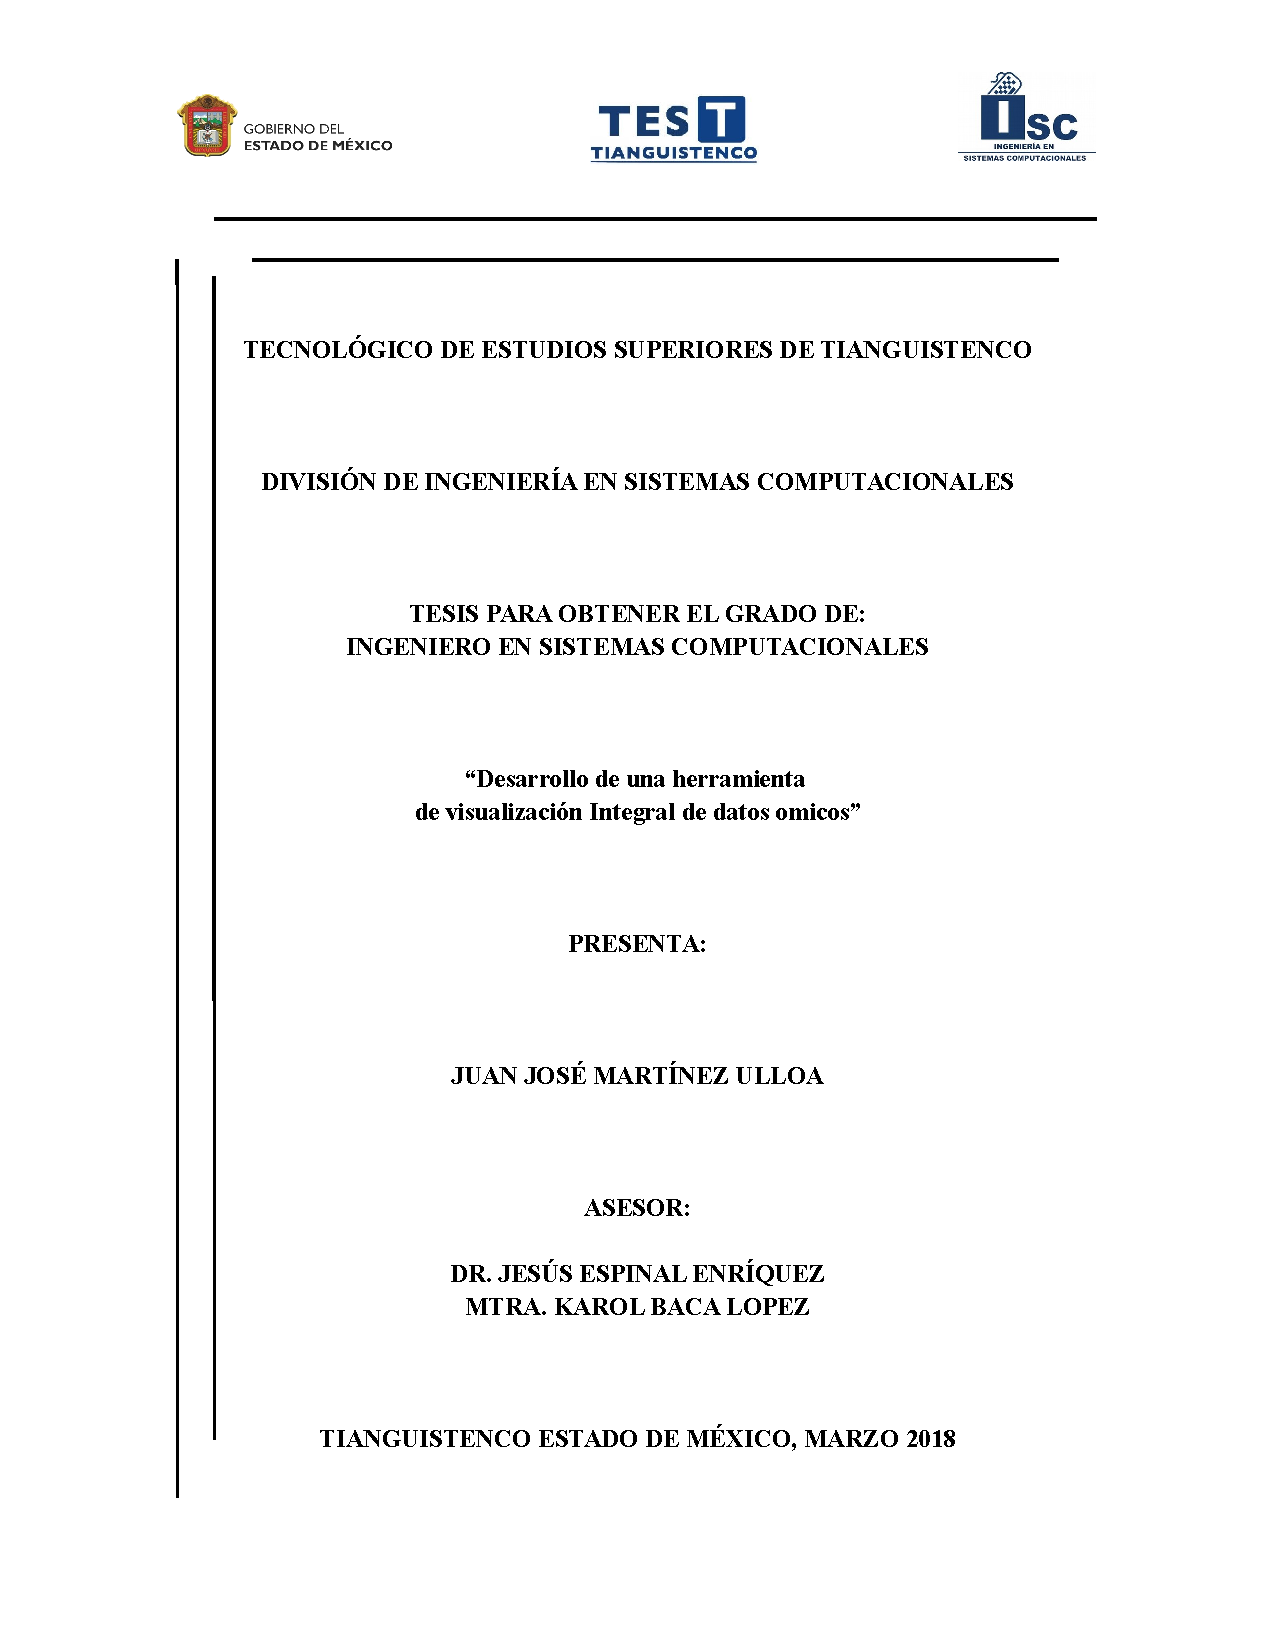
\includepdf[pages=1]{PORTADA}
\section*{Resumen.}
\section*{Abstract.}
\section*{Agradecimientos.}
\tableofcontents % indice de contenido
\section{Introducción}
\subsection{Planteamiento del Problema}
El cáncer de mama es una enfermedad compleja y heterogénea con más de 1,300,000 casos y 450,000 muertes cada año en todo el mundo. Esta enfermedad se caracteriza por diferentes ápectos biológicos como desregulazación de la expresión génica, alteraciones genómicas del ADN, etc. Todo esto da lugar al inicio y desarrollo del carcinoma de mama. En éstos últimos años el uso de datos ómicos, como los basados en  microarreglos (microarrays) y secuenciación, esta en su pleno () en el campo de la biomedicina. Todos estos datos permiten estudiar enfermedades desde un punto de vista biomolecular. Con esto, se ofrecen grandes oportunidades para mejorar tanto la comprención de la enfermedad, como el desarrollo de nuevos métodos para el diagnóstico y tratamiento del paciente, sin embargo, el análisis de estos datos producidos por estas tecnologías, es bastante complejo por lo que es necesario la aplicación de avanzadas técnicas de análisis y cálculos computacionales que permiten obtener la información biológica disponibles. Hasta el día de hoy todos estos datos óptenidos de diversos experimentos, datos de muy alta calidad, datos clinicamente bien anotados, y una gran cantidad de datos de canceres analizados con el fin de encontrar anomalias recurrentes que sean importantes de la enfermedad y estos datos se guardan en diversas plataformas que permiten tener uns gran cantidad de información , pero estos datos no son tan faciles de analizar, por ello, la bioinformática ayuda a manejar estructurar y organizarla para que sea mas fácil de comprender. Circos plot es una de las herramientas que existen para la visualización datos, ideal para explorar las relaciones entre objetos y posiciones. Esta herramienta es flexible, aunque originalmente fue diseñado para visualizar datos genómicos , se puede crear figúras a partir de datos en cualquier campo, desde la genómica hasta la visualización de la migración al arte matemático. Esta herramienta puede ser automatizada. Está controlado por archivos de configuración de texto plano, lo que lo hace díficil su incorporación en \textit{pipeline} de adquisición de datos, análisis e informes. Todo esto hace dificil su utilización en instalacion y desarrollo de la visualización. 
\subsection{Justificación}
La cantidad de información generada a través de las tecnologías de secuenciación masiva son enormes. La integración de toda esa información puede ayudar a tomar decisiones de índole biomédica e incluso clínica. 
Aunque existen plataformas ya conocidas capaces de presentar esa información de un modo amigable, la programación de dichas herramientas continúa siendo complicada para un usuario final. Es por esto, que generar una herramienta con gran capacidad de visualización, integración de información y facilidad de implementación para un usuario final es de la mayor importancia. 

Con el fin de mejorar el rendimiento y la cantidad de tiempo de los investigadores del Instituto Nacional de Medicina Genómica, es fundamental sistematizar este software para reducir el tiempo de programación y la investigación.
La sistematización 	de circos plot, brindará la posibilidad de que el investigador ahorre en tiempo de programación o en dado caso que no se conozca nada del uso nativo de circos plot, leer todo el manual de uso de dicho software, para que ocupe su mayor de tiempo en la investigación y solo tome varios minutos para diseñar su grafica circular llamada circos plot.


%Agregarlos a otros flujos de trabajo
%A la fecha se utilizaban 2 platoformas pero con el desarrollo se implementaran 4 
\subsection{Delimitación}
El desarrollo de tecnologías de secuenciación masiva es abrumador. Para poder integrar toda la información proveniente de dichas tecnologías es necesario contar con herramientas adecuadas para la obtención, análisis y visualización de las tecnologías anteriormente mencionadas.

Ante esta problemática, resulta altamente relevante generar una herramienta capaz de condensar en un solo golpe de vista varias capas de información, para que, de este modo, se pueda analizar con un mayor detalle los datos obtenidos.

Circos plot es una herramienta de apoyo visual que permite lograr la visualización a nivel de genoma completo varios tipos diferentes de datos: Expresión, mutaciones, metilación, citobandas, etc., de una manera amigable para el usuario final. 

Aunque circos plot tiene grandes ventajas en cuanto a la visualización, su programación es altamente complicada, por lo que generar un back-end que integre de modo sencillo varios tipos de datos, será de la mayor utilidad. 

\subsection{Hipótesis}
El desarrollo de una herramienta de Visualización integral permitirá el análisis de la información de los datos derivados de múltiples plataformas.
\subsection{Objetivos}
\subsubsection{Objetivo General}
Implemetar una herramienta de visualización que integre datos genómicos derivados de múltiples plataformas.
\subsubsection{Objetivos Específicos}
\begin{itemize}
\item Realizar el pretatamiento de los datos de trascriptoma (Microarreglos).
\item Realizar el pretatamiento de los datos de Metilación.
\item Desarrollar algoritmo computacional para hacer la búsqueda en la referencia del genoma humano con los datos de trascriptoma y metilación.
\item Desarrollar software para preprocesar datos de distintos tipos de tecnologías genómicas.
\item Desarrollar software para integrar al backbone de circos plot varias capas de información proveniente del paso anterior.
\item Generar opciones de visualización de fácil manejo para el usuario final.

\end{itemize}
\subsection{Aportaciones de la tesis}
La presente Tesis aportara
\section{Estado del Arte}
\section{Tecnologías genómica.}
Las tecnologías genómicas es el conjunto de herramientas orientadas al estudio integral del funcionamiento, contenido,  evolución del genoma. Es una de las áreas más vanguardistas de la biología. La genómica usa conocimientos derivados de distintas ciencias como la biología molecular, la bioquímica, la informática, la estadística, las matemáticas y la física.
Para entender un poco más de estas tecnologias y de los datos que se obtiene de las antes mencionadas, hablaremos de las tecnologias genómicas que son: Microarreglos y Metilación.
\section{Microarreglos}
Un microarreglo de ADN (ácido desoxirribonucleico) tambien llamado DNA chip, tambien llamado \textbf{oligonucleotido de DNA chip o gene chip} que consiste en pequeños fragmentos de ADN de los cuales representa un gen diferente \cite{VallinPlous2007}, es una superficie sólida a la cual se une una colección de fragmentos de ADN. Las superficies empleadas para fijar el ADN son muy variables y pueden ser de vidrio, plástico e incluso de silicona. Los chips de ADN se usan para analizar la expresión diferencial de genes.  Su funcionamiento consiste, básicamente, en medir el nivel de hibridación entre la sonda específica (probe, en inglés), y la molécula diana (target), y se indican generalmente mediante fluorescencia y a través de un análisis de imagen, lo cual indica el nivel de expresión del gen.	\\
Por lo tanto, los microarreglos son una potente fuente de obtención de perfiles de expresión de genes sometidos a diferente condiciones. Identificar los patrones de los niveles de expresión será muy útil para compararlos y poder estudiar las respuestas de los genes. \\
Aplicando una serie de procesos experimentales y computacionales sobre los microarreglos se obtiene una una matriz numerica bidimensional que consta de los genes de poblaciones distintas como individuos y de las condiciones experimentales a las que expusieron as células como variables en el caso que se quiera estudiar a los genes, o a la inversa, si es que se quiere realizar un estudio comparativo de las condiciones a que se somete. Cada uno de los valores de la matriz representa el nivel de expresión de un determinado gen bajo una cierta condición experimental. \\
Estas matrices son de grandes dimensiones puesto que existen una gran cantidad de condiciones experimentales y genes. En la figura 1 se puede observar el modelo de la presentación de los microarreglos. Cada fila representa un gen, el cual debe de ser indicado, cada columna represnta una condición experimental, cuyo nombre tambien debe de ser identicado. Los valores de la matriz son los niveles de expresión de los genes para la condicion experimental.
\begin{figure}[H]
\begin{center}
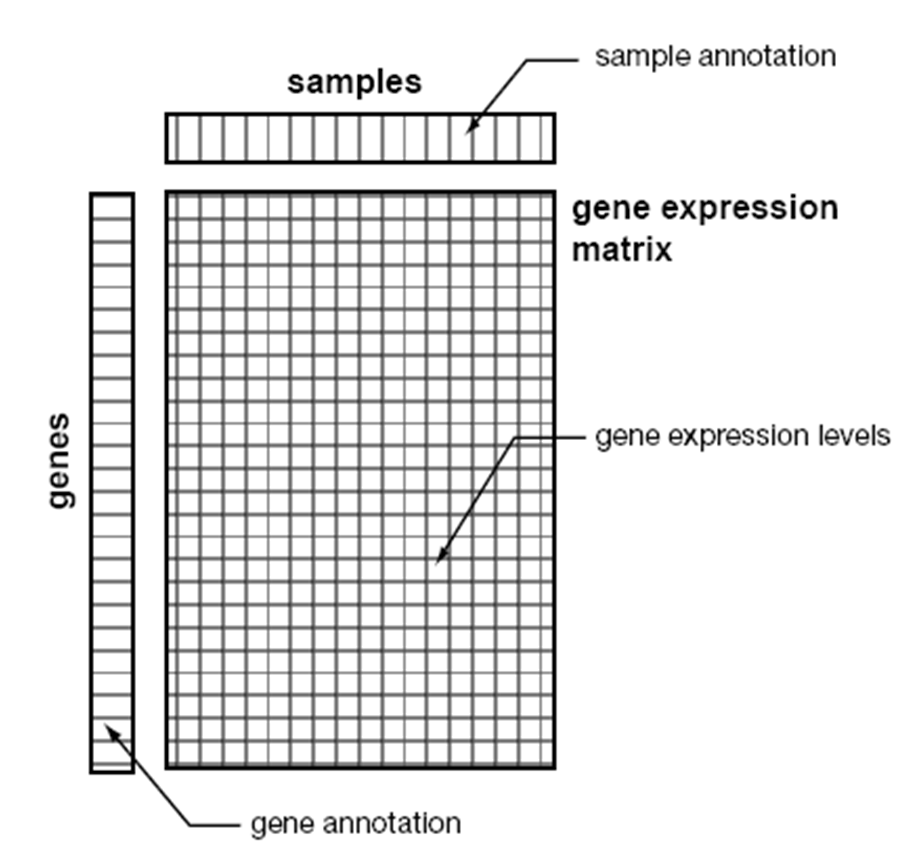
\includegraphics[width=0.7\textwidth]{matrix.png}
\end{center}
\caption{Chip de un Microarreglo}
\end{figure}
Dado que realizar un análisis de estas matrices de grandes dimensiones es una tarea prácticamente imposible, se hace necesarias técnicas computacionales que permitan analizar todos estos datos y entonces realizar el análisis biológico.\\
Actualmente existen diferentes bases de datos a nuestro alcance a través de Internet que unifican y facilitan toda esta información genética además de ofrecer diversas herramientas para el análisis de esta gran cantidad de información. Algunas de estas bases de datos por ejemplo son las que hay en el EMBL (European Molecular Biology Laboratory), el SIB (Swiss Institute of Bioinformatics), el EBI (European Bioinformatics Institute) o el NCBI (National Center for Biotechnology Information). El EBI y el NCBI son los que más información contienen y por lo tanto los más utilizados.
El tamño de los microarreglos es de 1.28 cm x 1.28 cm, hay 500,000 ubicaciones en cada matriz y por lo general tiene millones de cadenas de ADN construidas en cada ubicación, cada cadena contiene 25 pares bases (Figura 1).
\begin{figure}[H]
\begin{center}
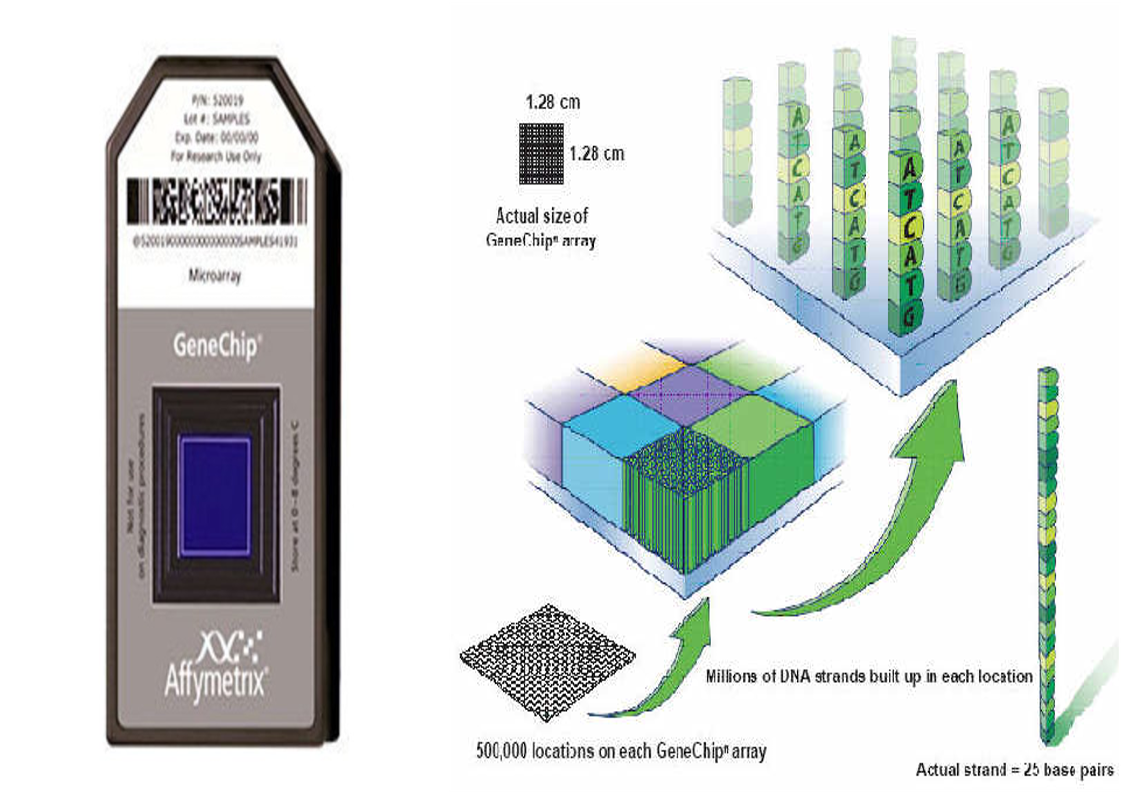
\includegraphics[width=0.7\textwidth]{Genechip.png}
\end{center}
\caption{Chip de un Microarreglo.}
\end{figure}
En estos chips se imprimen las secuencias biologicas en un chip, de manera que se puede cuantificar el transcripción en una matriz numérica.	
\subsection{Formato}
Los archivos están disponibles en un formato de valores separados por comas (CSV). Estos son archivos de texto sin formato con cada fila terminada por un carácter de nueva línea. Los datos en campos separados están entre comillas y separados por comas. Ninguno de los campos de datos contiene ninguno de estos caracteres: comillas, nueva línea, retorno de carro o tabulación.\\

Estos archivos se usen principalmente en aplicaciones de hojas de cálculo y programas de bases de datos (como bases de datos SQL). Los datos estan formateados de tal manera que estos dos usos sean relativamente fáciles. Se tiene en cuenta que algunos de los archivos y los campos de datos en ellos son grandes. 

La primera fila de cada archivo contiene los títulos de los campos que figuran en las filas siguientes.\\

Cada fila después de la primera fila contiene anotaciones para un solo conjunto de sondas. Todas las anotaciones para ese conjunto de sonda están contenidas en esa única fila. En algunos campos, como las anotaciones de dominio de proteínas, puede haber más de una anotación para un único conjunto de sondas. En este caso, los valores múltiples están separados por la cadena '///'.\\

En muchos tipos de anotaciones, los subcampos están separados por '//'. Por ejemplo,  una anotación para un "GO Biological Process" puede aparecer como "7155 // cell adhesion // predicted / computed".  En este caso, las secciones corresponden a "ID // Descripción // Evidencia", pero el significado de los subcampos varía entre los diferentes tipos de anotación, como se describe a continuación.\\

Los campos vacíos se indican con '- - -' . El hecho de utilizar una cadena de este tipo en lugar de dejar el campo vacío es que hace que la naturaleza columnar de los datos sea más visible en ciertos programas de hoja de cálculo.
Algunas columnas en algunos archivos no contienen datos. Para ayudar a los usuarios a combinar datos de varios archivos, dichas columnas vacías no se eliminan. Por lo tanto, cada archivo tiene las mismas columnas en el mismo orden.\\

Algunos campos, como "Chip", contienen el mismo valor para cada conjunto de sonda en un archivo. Aunque estos datos son redundantes en cualquier archivo individual, son útiles para los usuarios que combinan datos de varios archivos.
\subsection{Metilación}
La metilación es un proceso epigenetico que participa en la regulacion de la expresión genica de dos maneras, direcatmente al impedir de la unión de factores de transcripción, e indirectamente proporcionando la estructura "cerrada" de la cromatina\cite{Mesa-Cornejo, Viviana Matilde, Barros-Núñez, Patricio, & Medina-Lozano, Claudina2006}.

\begin{thebibliography}{XXX0000}
  \bibitem{VallinPlous2007} Microarreglos de ADN y sus aplicaciones en investigaciones biomédicas. Revista CENIC. Ciencias Biológicas, 38 (2), 132-135. 
  \bibitem {Mesa-Cornejo, Viviana Matilde, Barros-Núñez, Patricio, & Medina-Lozano, Claudina2006} Metilación del ADN: marcador diagnóstico y pronóstico de cáncer. Gaceta médica de México, 142(1), 81-82. 
\end{thebibliography} 	
\end{document}
